\documentclass[10pt]{beamer}
\setbeamerfont{structure}{family=\rmfamily} 
\usepackage{amsthm}
\usepackage{graphicx}
\usepackage{graphics}
\usepackage{hyperref}
\beamertemplatenavigationsymbolsempty
\setbeamertemplate{blocks}[rounded][shadow=true]
\setbeamertemplate{bibliography item}[text]
\setbeamertemplate{caption}[numbered]
\usetheme{default} 
\usecolortheme{seahorse}
\mode<presentation>
{
   \setbeamercovered{transparent}
   \setbeamertemplate{items}[ball]
   \setbeamertemplate{theorems}[numbered]
   \setbeamertemplate{footline}[frame number]

}

\begin{document}
\title {\bfseries{\sc Standalone Android Mobile Attendance Application }}
\author[Aaditya Menon and Abhishek Lal B]{\small {Aaditya Menon(AM.EN.U4CSE15001)\\Abhishek Lal B(AM.EN.U4CSE15002)\\Project Guide:\\Mr. Pradeesh Narayan\\Amrita E-learning Department\\Internal Guide:\\Mrs. Pratibhamol CP\\Assistant Professor, Dept. of Information Technology}}
\institute{
% commented by KK (put image if you want)
%\includegraphics[scale=.08]{Amrita.jpg}\medskip\\ 
\sc{Department of Computer Science \& Engineering}\\  \medskip\sc{Amrita School of Engineering}\\ \medskip \sc{\small Amrita Vishwa Vidyapeetham}}
\date{\small 6th April, 2019} 
%--------------------------------------------------------------------------%
\begin{frame}
\titlepage
\end{frame}
%---------------------------------------------------------------------------%
\section*{OUTLINE}
\begin{frame}
\frametitle{OUTLINE}  
\tableofcontents
\end{frame}
%---------------------------------------------------------------------------

\section{Problem Definition}
\begin{frame}
\frametitle{Problem Statement}
To implement an Android application for performing automatic group attendance system inside a classroom in a cost effective way.
\end{frame}
%---------------------------------------------------------------------------%
\section{Problem Description}
\begin{frame}
\frametitle{Problem Description}
\begin{itemize}
\item Abhishek fill this slide
\item InsideView gets News articles from News Providers like MoreOver.
\item Company News Pairing
\begin{itemize}
\item Company News has been extracted from news xml file.(by appling filter)
\item News which belongs to a particular company is paired.
\end{itemize}
\item entity-Relationship Extraction
\begin{itemize}
\item For getting entity relationship, Extract Name of the executives and their useful information (Designation, College from where they completed their degree etc), Company names.
\item With the help of these information form 1-degree, 2-degree connections.
\item These connections are changed according to environment.
\end{itemize}
\end{itemize}
\end{frame}
%-------------------------------------------------------------------------------%
\section{Work Done so far}
\subsection{Resolution Analysis}
\subsection{Face Detection and Recognition}
\begin{frame}
\frametitle{Modules in the Project}
\begin{itemize}
\item{\textcolor{red}{Resolution Analysis Module}} \\
\item{\textcolor{red}{Face detection and recognition module}}\\
\item{\textcolor{red}{Camera live-tracking module}} \\
\item{Attendance Marking on Phone Module}\\
\item{Sending data to server}\\
\end{itemize}
\end{frame}
\begin{frame}
\frametitle{Resolution Analysis}
\begin{itemize}
\item{Abhishek Ith thallu}
\end{itemize}
\end{frame}
%
\begin{frame}
\frametitle{Face Detection and Recognition}
%\includegraphics[scale=.23]{FlowChart.jpg}\\
\begin{itemize}
        \item {Add person to Training set}
        \item {Add person to Test set}
        \item {Recognition Training}
        \item {Validate Accuracy with Test set}
        \item {Detection View}
        \item {Recognition View}
\end{itemize}
\end{frame}

%--------------------------------------------------------------------------------------%
\section{Complete System design}
\begin{frame}
\frametitle{System Design - Resolution Analysis}
\begin{itemize}
    \item{Abhishek Ith thallu}
\end{itemize}
\end{frame}
\begin{frame}
\frametitle{Face Detection and Recognition Design}
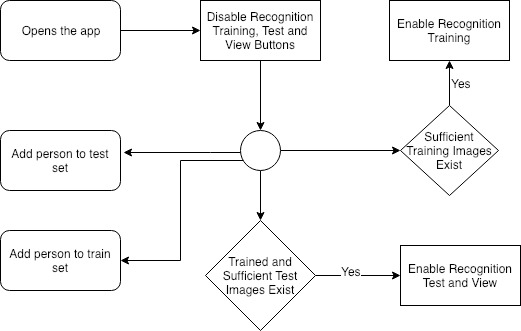
\includegraphics[scale=.5]{MainActivity.jpg}\medskip\\

\end{frame}
\begin{frame}
\frametitle{Add Person to Train/Test Set Design}
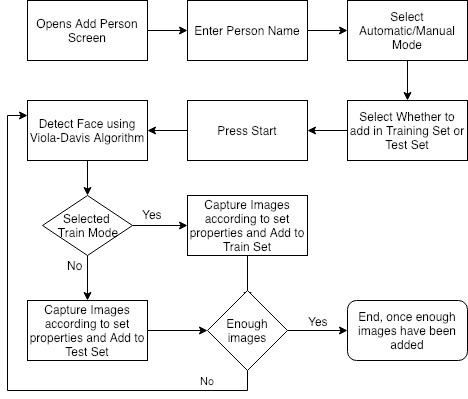
\includegraphics[scale=.6]{AddImages.jpg}\medskip\\

\end{frame}
\begin{frame}
\frametitle{Recognition Training Design}
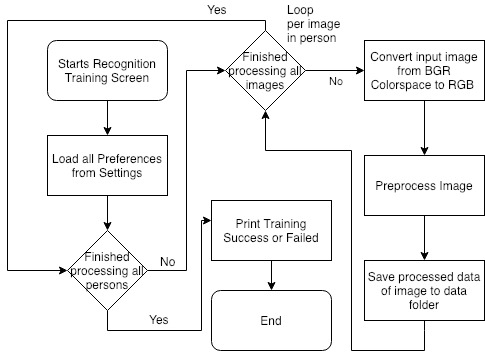
\includegraphics[scale=.55]{RecognitionTraining.jpg}\medskip\\
% Preprocessing - Detect Faces, Get Angle, Eye Detection, Brightness, Contrast, Contours
\end{frame}
\begin{frame}
\frametitle{Recognition Test Design}
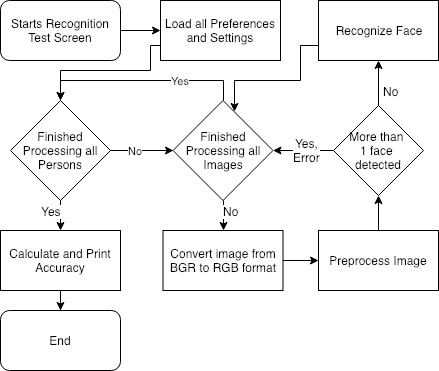
\includegraphics[scale=.55]{RecognitionTest.jpg}\medskip\\
% Preprocessing - Detect Faces, Get Angle, Eye Detection, Brightness, Contrast, Contours
\end{frame}
\begin{frame}
\frametitle{Library Architecture}
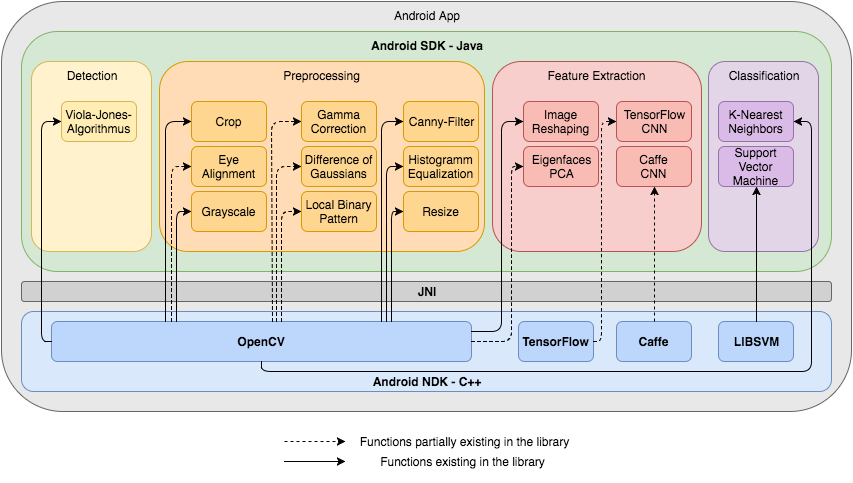
\includegraphics[scale=.38]{AppArchitecture.png}
\end{frame}
\begin{frame}
\frametitle{Viola-Jones algorithm for Face Detection}
\begin{itemize}
    \item{Used for face detection process}
    \item{Basic Steps:}
    \begin{itemize}
        \item{Integral Image for feature Computation}
        \item{Adaboost algorithm for feature selection}
        \item{Cascade Classifiers}
    \end{itemize}
    
\end{itemize}
\end{frame}
%-------------------------------------------------------------------------------------------------------%


%---------------------------------------------------------------------------%

%---------------------------------------------------------------------------%


\begin{frame}{References}
  \begin{thebibliography}{99}
  \bibitem{one}
Anis Das Sharma, Alpa Jain, Kong Yu, " Dynamic Relationship and Event Discvery".
\bibitem{two}
Nguyen Bach and Sameer Badaskar, Presentation on "Survey on Relation Extraction".
\bibitem{three}
Sunita Sarawagi, "Surv"

\end{thebibliography}
\end{frame}
%---------------------------------------------------------------------------%

\begin{frame}
\Large
\begin{center}
 \sc {Thank You \ldots} 
\end{center}
\end{frame}
%---------------------------------------------------------------------------%
\end{document}

